\documentclass[12pt,letterpaper]{article}
\usepackage[latin1]{inputenc}
\usepackage{amsmath, amsfonts, amssymb} % for equations
\usepackage{graphicx} % for inserting figures

% the above packages are the "base"

\usepackage{hyperref} % enable links within pdf
\hypersetup{colorlinks = true, linkcolor = black, urlcolor = blue}

\usepackage{float} % to fix the position of figures using [H]

% in-text citation styles
\usepackage[sort]{natbib}
\bibpunct[; ]{(}{)}{;}{a}{,}{;}

%  You "comment out" lines with the % symbol.



\title{\textbf{Introduction to ImageJ}\\Measuring Urchins in Photo Plots}

\author{} % insert your name here to have it appear

%\date{} % uncomment to have the date appear




\begin{document}

\maketitle

\tableofcontents

\pagebreak


\section{Downloading ImageJ}
\label{sec:download} % labels allow automatic referencing

Go to	{ImageJ (source: \url{https://imagej.net/ij/download.html})}

Follow instructions for Mac or Windows. For Macs, you may need to right click to open the downloaded file or it may not be trusted by your machine. 

\section{Protocol}

\subsection{Download photo from Box}

Go to Box and download your photo plot.	{(source: \url{https://oregonstate.app.box.com/folder/294649331958})}



\subsection{Open photo in ImageJ}

File and Open and select the phot you want to analyze. 



\subsection{Set the measurement scale}

Select the line tool from the toolbar and draw a line between two points of known distance. In this case, each photo has the quadrat in it. The quadrat is 50cm by 50cm. Draw a line that spans the length of the quadrat. Go to Analyze and Set Scale. In the Set Scale window, type the known distance (50) and the units of measurement (centimeter) in the appropriate boxes and click OK


\subsection{Set the measurement to area}

Go to Analyze and Set Measurement. In the Set Measurement window, select Area


\subsection{Within-text referencing}

I can easily reference the section (sect.\ref{sec:intro}), equation (eqn. \ref{eqn:calculus}) and table (Table \ref{tab:mytable}).
Their numbers will auto-generate, which makes it easy to move them around in your paper and adhere to
a journal's stylistic preferences.



\subsection*{My un-numbered subsection}

Sections and subsection are numbered by default, but that can be overwritten for a given section, or globally using \verb+\setcounter{secnumdepth}{0}+ in the preamble.




\section{More equations}

\subsection*{Using align}

The Lotka-Voltera equations are given by
\begin{align}
\frac{dx}{dt} 	&=	\alpha x - \beta xy \\
\frac{dy}{dt}	&=	\gamma xy - \delta y \,.
\end{align}

\noindent
Often it's useful to typeset the steps of derivations.
Pay it forward to folks who are trying to learn these methods, and to yourself when you can't remember the details but have to lecture on it in 5 minutes.
In these cases you don't need to number each line.

\begin{align}
N(10) 	&= 	\lambda N(9) 		\\ 		\notag
		&= 	\lambda^2 N(8) 	\\		\notag
		&=	\lambda^3 N(7) 	\\		\notag
		& \dots				\\		\notag
		&=	\lambda^{10} N(0) \,.	\\		\notag
\end{align}





\section{Inserting figures}

Note that the position of figures is auto-determined (e.g., Fig.~\ref{fig:logo})!
You can force the position of figures using the \texttt{float} package and then the [H] option for your figure (e.g., Fig.~\ref{fig:miktex}).

% Figures are included like this:
\begin{figure}
	\centering
	
\includegraphics[width=0.2\linewidth]{figs/LaTeX_logo.png}
	\caption{This is the \LaTeX~logo.}
	\label{fig:logo}
\end{figure}

\begin{figure}[H]
	\centering
	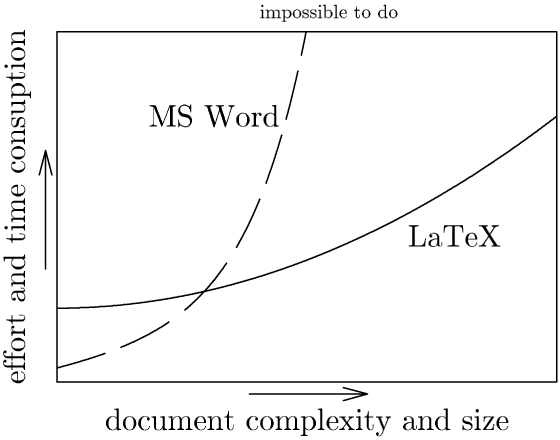
\includegraphics[width=0.8\linewidth]{figs/miktex.png}
	\caption{Why use \LaTeX\ (source: \url{http://www.pinteric.com/miktex.html})}
	\label{fig:miktex}
\end{figure}





\section{Inserting external tables}

It's relatively easy to use the R \texttt{Hmisc} package to generate \LaTeX\ tables (see
\texttt{../R/ExportTable.R}) and then import them into your document using \texttt{input}.
Again, just like figures, their placement in the document is auto-determined.
If you provided a caption to the tables when generating their tex files in R, it's easy to reference them (Table \ref{tab:data} and \ref{tab:coefs}).


% Table created by stargazer v.5.2.3 by Marek Hlavac, Social Policy Institute. E-mail: marek.hlavac at gmail.com
% Date and time: Mon, Mar 03, 2025 - 10:38:13
\begin{table}[!htbp] \centering 
  \caption{} 
  \label{tab:data} 
\begin{tabular}{@{\extracolsep{5pt}}lccccc} 
\\[-1.8ex]\hline 
\hline \\[-1.8ex] 
Statistic & \multicolumn{1}{c}{N} & \multicolumn{1}{c}{Mean} & \multicolumn{1}{c}{St. Dev.} & \multicolumn{1}{c}{Min} & \multicolumn{1}{c}{Max} \\ 
\hline \\[-1.8ex] 
x & 6 & 0.443 & 0.212 & 0.191 & 0.723 \\ 
y & 6 & 2.024 & 1.409 & $-$0.083 & 3.676 \\ 
\hline \\[-1.8ex] 
\end{tabular} 
\end{table} 


% Table created by stargazer v.5.2.3 by Marek Hlavac, Social Policy Institute. E-mail: marek.hlavac at gmail.com
% Date and time: Mon, Mar 03, 2025 - 10:38:14
\begin{table}[!htbp] \centering 
  \caption{} 
  \label{tab:coefs} 
\begin{tabular}{@{\extracolsep{5pt}} ccccc} 
\\[-1.8ex]\hline 
\hline \\[-1.8ex] 
 & Estimate & Std. Error & t value & Pr(\textgreater \textbar t\textbar ) \\ 
\hline \\[-1.8ex] 
(Intercept) & $0.709$ & $0.568$ & $1.247$ & $0.228$ \\ 
x & $3.184$ & $1.064$ & $2.991$ & $0.008$ \\ 
\hline \\[-1.8ex] 
\end{tabular} 
\end{table} 





\section{References}

The \texttt{natbib} package is great for citing references.
Reformatting for a different journal is as easy as changing the arguments of a function.
How to cite references and include them in a bibliography is demonstrated in the accompanying
\texttt{manuscript.tex} template in the parent folder of these lecture notes.

\begin{figure}
	\centering
	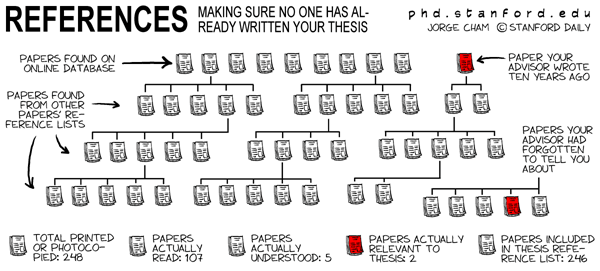
\includegraphics[width=1\linewidth]{figs/phd022702s.png}
	\caption{Reading is fundamental (source: \url{http://phdcomics.com/comics/archive.php?comicid=286})}
	\label{fig:phdrefs}
\end{figure}

\end{document}
